\documentclass[10pt,twocolumn,letterpaper]{article}

\usepackage{cvpr}
\usepackage{times}
\usepackage{epsfig}
\usepackage{graphicx}
\usepackage{amsmath}
\usepackage{amssymb}
\usepackage{natbib}

% Include other packages here, before hyperref.

% If you comment hyperref and then uncomment it, you should delete
% egpaper.aux before re-running latex.  (Or just hit 'q' on the first latex
% run, let it finish, and you should be clear).
\usepackage[breaklinks=true,bookmarks=false]{hyperref}

\cvprfinalcopy % *** Uncomment this line for the final submission

\def\cvprPaperID{****} % *** Enter the CVPR Paper ID here
\def\httilde{\mbox{\tt\raisebox{-.5ex}{\symbol{126}}}}

% Pages are numbered in submission mode, and unnumbered in camera-ready
%\ifcvprfinal\pagestyle{empty}\fi
\setcounter{page}{4321}
\begin{document}

%%%%%%%%% TITLE
\title{Comparing Pixel Inputs and Structured Inputs in Reinforcement Learning with Self-Play}

\author{Brendon Go\\
Stanford University\\
{\tt\small go@cs.stanford.edu}
% For a paper whose authors are all at the same institution,
% omit the following lines up until the closing ``}''.
% Additional authors and addresses can be added with ``\and'',
% just like the second author.
% To save space, use either the email address or home page, not both
\and
Evan Liu\\
Stanford University\\
{\tt\small evanliu@cs.stanford.edu}
}

\maketitle
%\thispagestyle{empty}

\section{Introduction}

In the Reinforcement Learning (RL) paradigm, agents learn to perform complex
tasks through trial-and-error. The agents take certain actions and observe their
consequences (reward) -- learning to prefer actions that lead to positive
consequences.  This paradigm has shown great promise in disparate
applications, ranging from dialogue generation \citep{dialogue2016}, to game
playing \citep{mnih2015human}, to robotics \citep{robotics2016}.

Recent RL methods have achieved superhuman performance on Atari 2600 games
\citep{bellemare2013arcade}. These methods receive as input the raw pixels that
appear on the game screen, and output actions (e.g. moving left or right),
learning to find action sequences that maximize the game score. Traditional
wisdom posits that the task would be easier if the input were structured (e.g.
the positions of the character and enemies in the game) rather than pixels,
because with pixel inputs, the pixels must first be processed to extract this
structured information. However, surprisingly, on a version of the Atari 2600
games, where the inputs to the RL agent are the game memory (which include
information like the coordinates of the avatar), current RL methods perform
poorly, far worse than on the pixel version \citep{atariRAM}.

We investigate this phenomenon on games outside of Atari to determine
if the poor performance is an artifact of the structure of Atari games or if
there is a deeper reason. In particular, we focus on a favorite game from the
90s, Slime Volleyball, where the goal of the game is to hit a ball over a net
onto the opponent's side of the game. Players win points when the ball hits the
ground on the opponent's side of the net. We apply deep RL methods to
this game with two types of inputs: the pixels of the game screen, and the
variables used to generate the game, and compare the performance of these
algorithms on different types of inputs. Success on this project will hopefully
lend greater insight into why Atari on RAM states fails, possibly leading to
novel RL algorithms or insights about the pixel states. In the process, we
also investigate into self-play methods in RL, (TODO: cite) which have shown
grown success in learning to solve complex tasks.

\section{Task}

We operate in a Markov Decision Process (MDP), consisting of the set of
possible states $\mathcal{S}$, the set of possible actions $\mathcal{A}$, the
reward dynamics $\mathcal{R}: \mathcal{S} \times \mathcal{A} \to \mathbb{R}$,
describing what rewards the agent receives when it plays a certain action in a
certain state, the environment dynamics $P: \mathcal{S} \times \mathcal{A}
\times \mathcal{S} \to \mathbb{R}$ describing the probability of transitioning
to a new state from the current state after taking an action, and a discount
factor $\gamma$. States $s \in \mathcal{S}$ are assumed to have the
Markov-property: the current state contains all of the necessary information to make
decisions. The goal is to learn a policy $\pi$ that maps a state to the action
to take in that state that maximizes the expected discounted reward.

In contrast to the traditional single-agent RL setup, which includes only a
single RL agent, our setting contains two RL agents that play against each
other. Notably, from the point of view of the first agent, the environment
dynamics function $P$ encodes the policy of the other agent -- when the other
agent's policy changes, the environment dynamics model also change. This means
that the environment dynamics model is non-stationary if both agents are
learning, and that the environment dynamics model differs between the points
of views of the first and second agents. This introduces additional technical
challenges addressed in (TODO: ref technical approach section).

\subsection{Slime Volleyball}


\begin{figure}[h]
\center
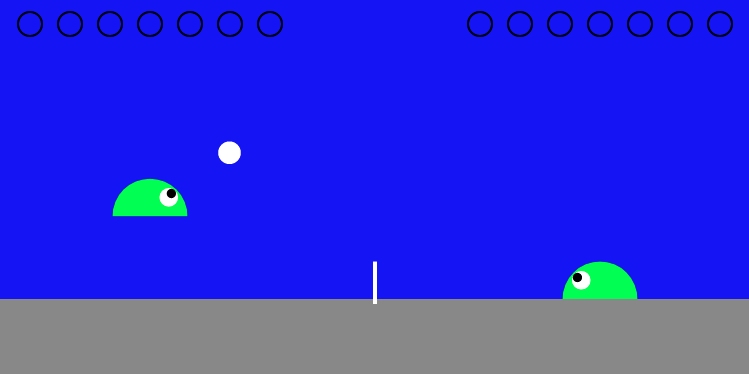
\includegraphics[width=\columnwidth]{SlimeVolleyBall}
\caption{
Player 1 Serving the ball over the net in Slime Volleyball
}\label{fig:slime}
\end{figure}


In Slime Volleyball, there are two agents, on either set of a volleyball net.
On each point, the agents attempt to hit the volleyball over the net to the
opponent's side. If the ball hits the ground on the opponent's side, the agent
wins the point and receives reward $+1$. If the ball hits the ground on the
agent's side, the agent receives reward $-1$, and $0$ reward while the point
is still in play. The game terminates after either agent wins $7$ points. To
hit the ball, the agent can take actions of moving left, right, or jumping.
The ball bounces off the agent's head when the agent collides with the ball.
Notably, agents can jump as many times as they wish, and can also jump over
the net to the opponent's side of the net.

We have modified an HTML5 implementation of Slime Volleyball, to use
as a browser-based simulation environment. Following (TODO: cite), we use
Selenium to send actions to the browser simulation environment and receive
responses to update the agents. The browser simulation environment is
configured to run in two modes: pixel states and structured states. In the
pixel state mode, the agent receives as input the screenshot of the screen. In
structured state mode, the agent receives as input a structured list
consisting of the $(x, y)$ coordinates and velocity of the agent, the
opponent, and the ball, as well as the current score. Notably, the states are
configured such that reflecting the pixel or structured state for the first
agent over the x-axis results in the state of the second agent. This enables
us to maintain a single model act for both agents.

\subsection{Goal}

Our goal is to compare the performance of agents that use pixel state vs.
agents that use structured state. Concretely, we seek to answer the following
questions:

\paragraph{Training Speed and Asymptotic Performance without Self-Play.} In
Atari, we are surprised to find that models that use structured inputs far
underperform models that use pixel inputs. This may be due to some of the
intuitions that make SVMs work -- pixel inputs effectively project the
structured inputs to a much higher dimension to perform computation. We seek
to understand if this phenomenon holds in Slime Volleyball. To evaluate this,
we train a pixel-input agent and a structured-input agent against a
fixed random opponent. This attempts to isolate effects of self-play vs. the
effects of differing inputs. We report on sample efficiency (number of samples
to required to learn) and asymptotic performance (average episode reward after
training converges).

\paragraph{Performance with Self-Play.} We further are interested in the
effects of self-play combined with differing inputs. To evaluate this, we
propose to play an agent using pixel-inputs against an agent using
structured-inputs. We will use alternating optimization on each agent and
report on sample efficiency and asymptotic performance.

\paragraph{Comparison with Human Play.} Finally, we also want to compare our
models against humans. We propose not to directly optimize against human play,
but learn models via self-play. After many rounds of self-play, we will play
the trained models against humans and report the asymptotic performance.
Notably, humans might use strategies that are not seen during self-play.
Results could be particularly interesting if the models perform well even
against these novel strategies.

\section{Technical Approach}

\subsection{Deep Q-Learning}

We implement the policies for each agent as Deep Q-Networks (TODO:
cite). In Deep Q-Learning, a value function $Q(s, a)$ is learned that
estimates the discounted reward to go that the agent will receive for playing
action $a$ in state $s$ and continuing to follow its current policy. The
learned $Q$ function encodes a policy, which at each state $s$ plays the
action $a = argmax_{a \in \mathcal{A}}Q(s, a)$. Our $Q$ functions are
implemented as neural networks. For structured state inputs, the network
consists of several multi-layer perceptrons (MLP). For pixel state inputs, the
network consists of several convolutional layers, followed by a MLP. The
encoded policy can be made non-greedy by following an $\epsilon$-greedy
policy, which greedily chooses the best action $a$ according to $Q$ with
probability $1 - \epsilon$ and choosing a random action with probability
$\epsilon$. We utilize an $\epsilon$-greedy policy with an $\epsilon$ that
anneals to $0$ during training to ensure that the policy adequately explores
the state and action spaces.

Following (TODO: Cite), we make use of experience replay for learning $Q$. The
agent follows an the $\epsilon$-greedy policy recording all transitions $(s,
a, r, s')$ in a fixed-size replay buffer, where $s$ is the state, $a$ is the
action played in state $s$, $r$ is the received reward, and $s'$ is the
resulting new state. To update, several of these transitions are sampled and
the following loss function is optimized: $||Q(s, a) - (r + \gamma \max_{a'
\in A}Q(s', a'))||^2$. Experience replay enables updates with removed temporal
correlations. In addition, Q-learning requires many updates to ensure that
later $Q$ values propagate backwards to earlier $Q$ values. We also make usage
of double DQN (TODO: cite) so that the network that we max the actions over is
different from the network we utilize for updates.

\subsection{Self-Play}

As previously mentioned, when both agents are updating, the environment
dynamics appear non-stationary. Notably, in multi-agent systems, independent
Q-Learning (IQL), where each agent maintains its own $Q$ function fails
precisely because of the non-stationaryness (TODO: cite).  To get around this,
we use the following self-play algorithm. We keep track of the fixed best
current agent (initialized randomly). We match the best current agent against
a contender agent, which is optimized for a fixed number of episodes. If the
contender agent beats the current agent, then the contender agent becomes the
new best current agent, and a new contender is created. New contenders are
initialized from the parameters of the current best agent.

\section{Intermediate/Preliminary Results}

We have currently implemented the models described in the previous sections.
However, due to limited computational resources, we have limited experimental
results. We have shown that our models can successfully beat random agents $7$
to $0$. For the final project, we plan to continue implementing the self-play
algorithm we described and also run more experiments.

{\small
\bibliographystyle{unsrtnat}
\bibliography{egbib}
}

\end{document}
